\documentclass[11pt,a4paper]{article}

\usepackage[T1]{fontenc}
\usepackage[utf8]{inputenc}
\usepackage[english]{babel}
\usepackage[margin=2.4cm]{geometry}
\usepackage{amsmath,amssymb}
\usepackage{graphicx}
\usepackage{booktabs}
\usepackage{xcolor}
\usepackage[colorlinks=true,linkcolor=black,urlcolor=blue]{hyperref}
\usepackage{caption}
\usepackage{natbib}
\bibpunct{(}{)}{;}{a}{}{,}

\captionsetup{font=small,labelfont=bf}
\setlength{\parskip}{0.35em}

\renewcommand{\topfraction}{0.92}
\renewcommand{\bottomfraction}{0.85}
\renewcommand{\textfraction}{0.06}
\setcounter{topnumber}{3}
\setcounter{totalnumber}{4}
\usepackage[section]{placeins}

\newcommand{\Msun}{M_\odot}
\newcommand{\Req}{R_{\mathrm{eq}}}
\newcommand{\Epol}{E_{\mathrm{pol}}}
\newcommand{\Emag}{E_{\mathrm{mag}}}
\newcommand{\Pm}{\mathrm{Pm}}
\newcommand{\Rm}{\mathrm{Rm}}
\newcommand{\Rey}{\mathrm{Re}}
\newcommand{\lmri}{\lambda_{\mathrm{MRI}}}

\title{\textbf{The shearing box, and the three numbers that govern it}\\[0.3em]
\large Why the global runs cannot resolve the MRI; what $\Pm$, $\Rm$ and
$\alpha$ are; and what a scan over $\Pm$ measures\\[0.2em]
\normalsize Report III --- companion to \texttt{report\_rot192\_rot256} and
\texttt{report\_late\_convergence}}
\author{Rafael C.\ R.\ de Lima}
\date{9 August 2026}

\begin{document}
\maketitle

\begin{abstract}
\noindent
Reports I and II found that the differential rotation of a $2.005\,\Msun$
magnetised white dwarf is not erased, and steepens by $22.6\%$. Both are
bounded by one limitation: the magnetorotational instability is not resolved,
with a quality factor $Q = \lmri/\Delta x \simeq 0.4$ over the very window in
which the steepening is measured. This report sets out the route around that
limitation and the first results along it. A \emph{local} calculation can reach
what the global grid cannot, because in the incompressible approximation --- valid
here to $v/c_s \sim 4\times10^{-4}$ --- the acoustic timestep disappears and a
hundred orbits costs hours rather than months. Three dimensionless numbers govern
what such a box can say, and all three are defined and evaluated here for the
first time in this campaign. \textbf{The magnetic Prandtl number of the stellar
interior is $\Pm \approx 750$}, computed from electron transport in degenerate
matter --- not the $\Pm \sim 0.6$ of the cool crystallising white dwarfs in the
literature, and two orders \emph{above} rather than below the threshold at which
MRI turbulence is known to die. \textbf{The magnetic Reynolds number is the
campaign's central limitation}: the star sits at $\Rm \sim 10^{20}$ and our
global runs at $\Rm \approx 5$, a gap of twenty orders of magnitude that no
resolution we can afford closes. A scan of five box simulations over
$\Pm = 1$--$16$ finds transport rising as $\Pm^{0.19}$ and then flattening
above $\Pm = 8$; whether that flattening is physical or a resolution artefact
is not settled here. Either way the transport at the stellar $\Pm$ is
$1.6$--$3.7$ times the $\Pm = 1$ value --- a factor of a few, not orders of
magnitude, so it is $\alpha$ and not the Prandtl number that decides the
outcome. Converting the measured stress to the star gives
$\alpha \sim 8\times10^{-4}$. An envelope estimate put the braking time at
$130$\,s against a $78$\,s run; replacing it with an actual torque across the
half-mass radius gives $293$--$557$\,s, four times longer, so the rotation would
\emph{not} have been erased inside our run. What replaces that claim is sharper:
\textbf{the predicted MRI torque is $1.3$ times the angular-momentum transport
we actually observe, and opposite in sign.} The observed transport is inward and
produces the steepening; the MRI would drive it outward. It is a leading-order
competing effect of the same size, and whether the steepening survives it cannot
be settled by anything measured here.
\end{abstract}

%======================================================================
\section{Why a box at all}

Report~I states on its first page that the MRI is unresolved. The number is
worth repeating because everything here follows from it. Measured from the
volume-typical vertical field rather than its peak, the quality factor
$Q = \lmri/\Delta x$ peaks at $6.5$ near $t = 4.5$\,s and sits at $0.3$--$0.5$
over $t = 40$--$78$\,s. Representing the linear MRI mode needs $Q \gtrsim 6$;
converged turbulence needs $Q \gtrsim 15$--$20$, which this mesh never
approaches under any assumption.

Refining is not the answer. Cost scales as $N^4$ --- cells as $N^3$ and timesteps
as $N$ --- so the factor needed is prohibitive. What changes the problem is
dropping to a \emph{local} model and, with it, changing the equations.

\paragraph{The incompressible approximation, and why it is not a compromise
here.} In incompressible MHD the thermal pressure becomes a Lagrange multiplier
enforcing $\nabla\cdot\mathbf{v} = 0$, the sound speed is formally infinite, and
the acoustic constraint $\Delta t \le \mathrm{cfl}\,\Delta x/c_s$ vanishes. The
approximation is valid when both the flow and the Alfv\'en speed are far below
$c_s$. In our interior $v/c_s \sim 4\times10^{-4}$ and $v_A/c_s \sim 10^{-5}$, so
it is not marginally acceptable but ideal. The consequence is a factor
$c_s/v_{\mathrm{turb}} \sim 5\times10^4$ in the number of timesteps per orbit:
a compressible box needs $5\times10^6$ steps per orbit, an incompressible one
about $100$. Measured throughput is $80$\,s per orbit at $64^3$ on eight
threads, so a hundred orbits is about two hours.

A second consequence matters for interpretation: \textbf{the plasma $\beta$ does
not appear in the incompressible equations at all}. The $\beta \sim 10^9$ that
made a compressible box unaffordable was a property of the numerical method we
had chosen, not of the physics. What remains is the shear parameter $q$, the box
size in units of $\lmri$, and the numbers below.

\paragraph{What the box cannot do.} The Tayler instability, which is what
destroys the ordered field in the global runs, is driven by the curvature of
toroidal field lines about the rotation axis. A local Cartesian box has no
curvature, so the $m=1$ kink cannot grow there by construction. Nothing in this
report bears on the field-destruction result of Reports~I and II.

%======================================================================
\section{The three numbers}

\subsection{$\Pm$: which diffusion wins}

The magnetic Prandtl number is the ratio of two diffusivities, both in
cm$^2$\,s$^{-1}$:
\begin{equation}
  \Pm \;=\; \frac{\nu}{\eta},
\end{equation}
with $\nu$ the kinematic viscosity --- how fast \emph{momentum} spreads --- and
$\eta$ the magnetic diffusivity --- how fast the \emph{field} slips through the
fluid. It says nothing about how viscous or how resistive the material is, only
which of the two acts faster.

The physics is in which dissipation bites first as one goes to small scales.
At $\Pm \gg 1$ viscosity smooths the velocity field while the magnetic field
survives, so the field reaches scales \emph{smaller} than the motions that made
it. At $\Pm \ll 1$ the field leaks away before the velocity is damped, and one
can have vigorous turbulence that sustains no field at all --- which is why
liquid-sodium laboratory dynamos are so difficult. For the MRI this is decisive,
because the instability manufactures small-scale structure: whether it sustains
itself, and how much angular momentum it carries, depends on which dissipation
arrives first.

\subsection{$\Rm$: whether the field is carried or leaks}

The magnetic Reynolds number compares advection of the field against its
diffusion,
\begin{equation}
  \Rm = \frac{LV}{\eta},
  \qquad\text{alongside}\qquad
  \Rey = \frac{LV}{\nu},
  \qquad\text{so that}\qquad
  \Pm = \frac{\Rm}{\Rey}.
\end{equation}
At $\Rm \gg 1$ the field is frozen into the fluid in the sense of Alfv\'en's
theorem: field lines are dragged with the flow, and stretching or amplifying
them is a matter of moving the fluid. At $\Rm \lesssim 1$ the field diffuses out
faster than the flow can move it, and no amount of stirring will hold it.
Dynamos have a critical $\Rm$, typically $10$--$100$, below which no flow
sustains a field.

\subsection{$\alpha$: how much angular momentum the turbulence actually carries}

$\Pm$ and $\Rm$ say what regime the plasma is in. $\alpha$ is the answer one is
after: a dimensionless measure of \emph{transport efficiency}, introduced by
Shakura \& Sunyaev for accretion discs and used ever since as the single number
summarising what turbulence does to angular momentum. It is the turbulent stress
in units of the pressure,
\begin{equation}
  \alpha \;=\; \frac{W_{\varpi\varphi}}{P}
  \;=\; \frac{\big\langle \rho\, \delta v_\varpi\, \delta v_\varphi \big\rangle
              - \big\langle B_\varpi B_\varphi \big\rangle/4\pi}{P},
\end{equation}
Reynolds stress plus Maxwell stress over pressure, and it enters the dynamics
as an effective viscosity $\nu_t = \alpha\, c_s H$. Resolved MRI simulations
find $\alpha \sim 0.01$ without net flux and $\alpha \sim 0.1$--$1$ with it.

Two things about $\alpha$ matter here specifically.

\paragraph{An incompressible box cannot give $\alpha$ directly.} There is no
pressure in the incompressible equations, so the denominator does not exist.
What the box measures is the stress normalised by the imposed field, $W/B_0^2$,
and converting to $\alpha$ requires the star's own field and pressure:
\begin{equation}
  \alpha \;=\; \frac{2}{\beta}\,\frac{W}{B_0^2},
  \qquad \beta = \frac{P}{B_z^2/8\pi}.
  \label{eq:alpha}
\end{equation}
So $\alpha$ is small in our star not because the MRI is inefficient but because
the vertical field is weak relative to the pressure.

\paragraph{$\alpha$ is what sets the answer, and $\Pm$ only modifies it.} The
braking time of the differential rotation follows from $\nu_t$, so $\alpha$ is
the quantity that decides whether the rotation survives. The Prandtl number
enters only through the factor of a few by which it shifts $\alpha$ --- which is
why the modest $\Pm$ dependence measured in Section~5 is good news rather than a
disappointment.

\subsection{Why $\Rm$ is this campaign's central limitation}

Table~\ref{tab:rm} is, in one place, the reason the global results are bounded.

\begin{table}[h]
\centering\small
\begin{tabular}{llr}
\toprule
& & $\Rm$ \\
\midrule
The star & degenerate matter, $\eta = 3.3\times10^{-3}$\,cm$^2$/s & $\sim 10^{20}$ \\
Our $192^3$ run & set by the mesh & $\approx 3$ \\
Our $256^3$ run & set by the mesh & $\approx 6$ \\
The box, this report & set by us, explicitly & $10^3$--$1.6\times10^4$ \\
\bottomrule
\end{tabular}
\caption{The star is effectively perfectly conducting, with an ohmic decay time
of order $10^{10}$ years. Our global simulations behave as though the matter
were twenty orders of magnitude more resistive. This is not a modelling choice:
the mesh itself diffuses field, with a numerical diffusivity
$\eta_{\mathrm{num}} \approx 0.6$--$0.9\,c_s\Delta x$ extracted from the
measured decay, and it cannot be switched off.}
\label{tab:rm}
\end{table}

Two things follow. First, at $\Rm \approx 5$ the global runs are not in
quasi-ideal MHD but in a \emph{diffusive} regime, so ``the ordered field is
destroyed'' mixes a real $m=1$ instability with mesh leakage, and two
resolutions cannot separate them. Second, this is why a large-eddy treatment was
rejected: such models represent a turbulent cascade continuing below the cell,
and at $\Rm \approx 5$ there is no cascade to represent.

The box inverts the situation. There $\Rm$ is \emph{explicit} --- written into the
input file and enforced by a physical resistivity well above the numerical
one --- which is precisely why a local calculation can measure what the global run
cannot.

%======================================================================
\section{The stellar $\Pm$}

Electron transport dominates in degenerate matter. Following
\citet{shternin2008}, the shear viscosity is
\begin{equation}
  \eta_{\mathrm{visc}} = \frac{n_e v_F p_F}{5\,\nu_e},
  \qquad \nu_e = \nu_{ee} + \nu_{ei},
\end{equation}
and the asymmetry that fixes $\Pm$ is that electron--electron collisions
conserve the total electron momentum. They therefore do \emph{not} degrade a
current and stay out of the electrical conductivity, while they \emph{do}
degrade shear stress and enter the viscosity. Hence
$\sigma = n_e e^2/(m^\ast \nu_{ei})$ with $\nu_{ei}$ alone, and
$\eta = c^2/4\pi\sigma$.

At the run's mean density $\rho = 4.8\times10^{7}$\,g\,cm$^{-3}$ and an assumed
remnant temperature $T = 10^8$\,K, this gives $\nu = 2.4$ and
$\eta = 3.3\times10^{-3}$\,cm$^2$\,s$^{-1}$, so
\begin{equation}
  \boxed{\Pm \approx 750.}
\end{equation}
The result is robust: $\Pm$ stays above $190$ across
$\rho = 5\times10^7$--$10^9$ and $T = 10^7$--$10^9$\,K, and above $30$ even for
a Coulomb logarithm of $5$. Reaching $\Pm = 1$ would need a Coulomb logarithm
near $27$, which is unphysical. The ions are a liquid throughout
($\Gamma = 13$, melting near $175$), and electron--ion scattering dominates
($\nu_{ee}/\nu_{ei} = 0.04$).

\paragraph{This corrects a value taken from the literature.} A figure of
$\Pm \sim 0.6$ circulates for white dwarfs and was used earlier in this
campaign. It is quoted for the convective region of a \emph{cool crystallising}
CO white dwarf --- a much lower density and temperature, and plausibly a regime
where ion rather than electron viscosity dominates. It does not describe a hot
$2\,\Msun$ merger remnant.

The correction matters twice over, and in our favour both times. The threshold
below which MRI turbulence dies, $\Pm_{\mathrm{crit}} \sim 2$--$4$, is no longer
a concern: we are two to three orders \emph{above} it. And we sit in the same
high-$\Pm$ regime as the protoneutron-star boxes in which published subgrid
closure coefficients were calibrated, so those coefficients have a far better
chance of transferring than had been feared.

\paragraph{One assumption is unavoidable and should be visible.} The equation of
state used in the global runs is barotropic and carries no temperature at all,
so $T$ here is an assumption about a merger remnant rather than a simulation
output. That is why the calculation is presented as a scan rather than a single
value.

%======================================================================
\section{The scan}

Five incompressible shearing-box simulations with SNOOPY v6.0
\citep{lesur2007}, $64^3$, box $(4,4,1)$, net vertical flux $B_{z0} = 0.1$,
$\Rey = 1000$ fixed and $\Pm$ varied from $1$ to $16$, each run to $31.8$
orbits with $1401$ samples averaged over $t > 60$.

Keplerian shear $q = 1.5$ was used deliberately, rather than our star's
$q = 0$--$2$. It is where $\alpha(\Pm)$ has been published, so the same runs
measure the trend and check our use of the code against numbers obtained
independently. Scanning our own $q$ comes after that check; the other order
would leave any disagreement unattributable between a setup error and physics.

SNOOPY works in Alfv\'en units, so $b$ \emph{is} $v_A$ and the total
angular-momentum flux is $W = \langle v_x v_y\rangle - \langle b_x b_y\rangle$,
Reynolds plus Maxwell, the Maxwell term entering with a minus sign. There being
no sound speed in an incompressible box, the usual $\alpha = W/c_s^2$ is
meaningless and the net-flux normalisation $W/B_0^2$ is used instead.

\begin{table}[h]
\centering\small
\begin{tabular}{rrrrr}
\toprule
$\Pm$ & $W/B_0^2$ & Maxwell & Reynolds & Max/Rey \\
\midrule
$1$  & $19.32 \pm 0.21$ & $0.160$ & $0.0335$ & $4.76$ \\
$2$  & $22.67 \pm 0.26$ & $0.191$ & $0.0362$ & $5.26$ \\
$4$  & $25.24 \pm 0.30$ & $0.215$ & $0.0374$ & $5.74$ \\
$8$  & $\mathbf{31.84 \pm 0.33}$ & $0.271$ & $0.0479$ & $5.65$ \\
$16$ & $\mathbf{31.88 \pm 0.32}$ & $0.272$ & $0.0473$ & $5.74$ \\
\bottomrule
\end{tabular}
\caption{Transport against $\Pm$. The last two rows are indistinguishable.
Maxwell/Reynolds between $4.8$ and $5.7$ is above the $3$--$5$ of zero-net-flux
boxes and is what net flux is expected to give; it is a check on the setup, not
a result.}
\label{tab:scan}
\end{table}

\begin{figure}[h]
\centering
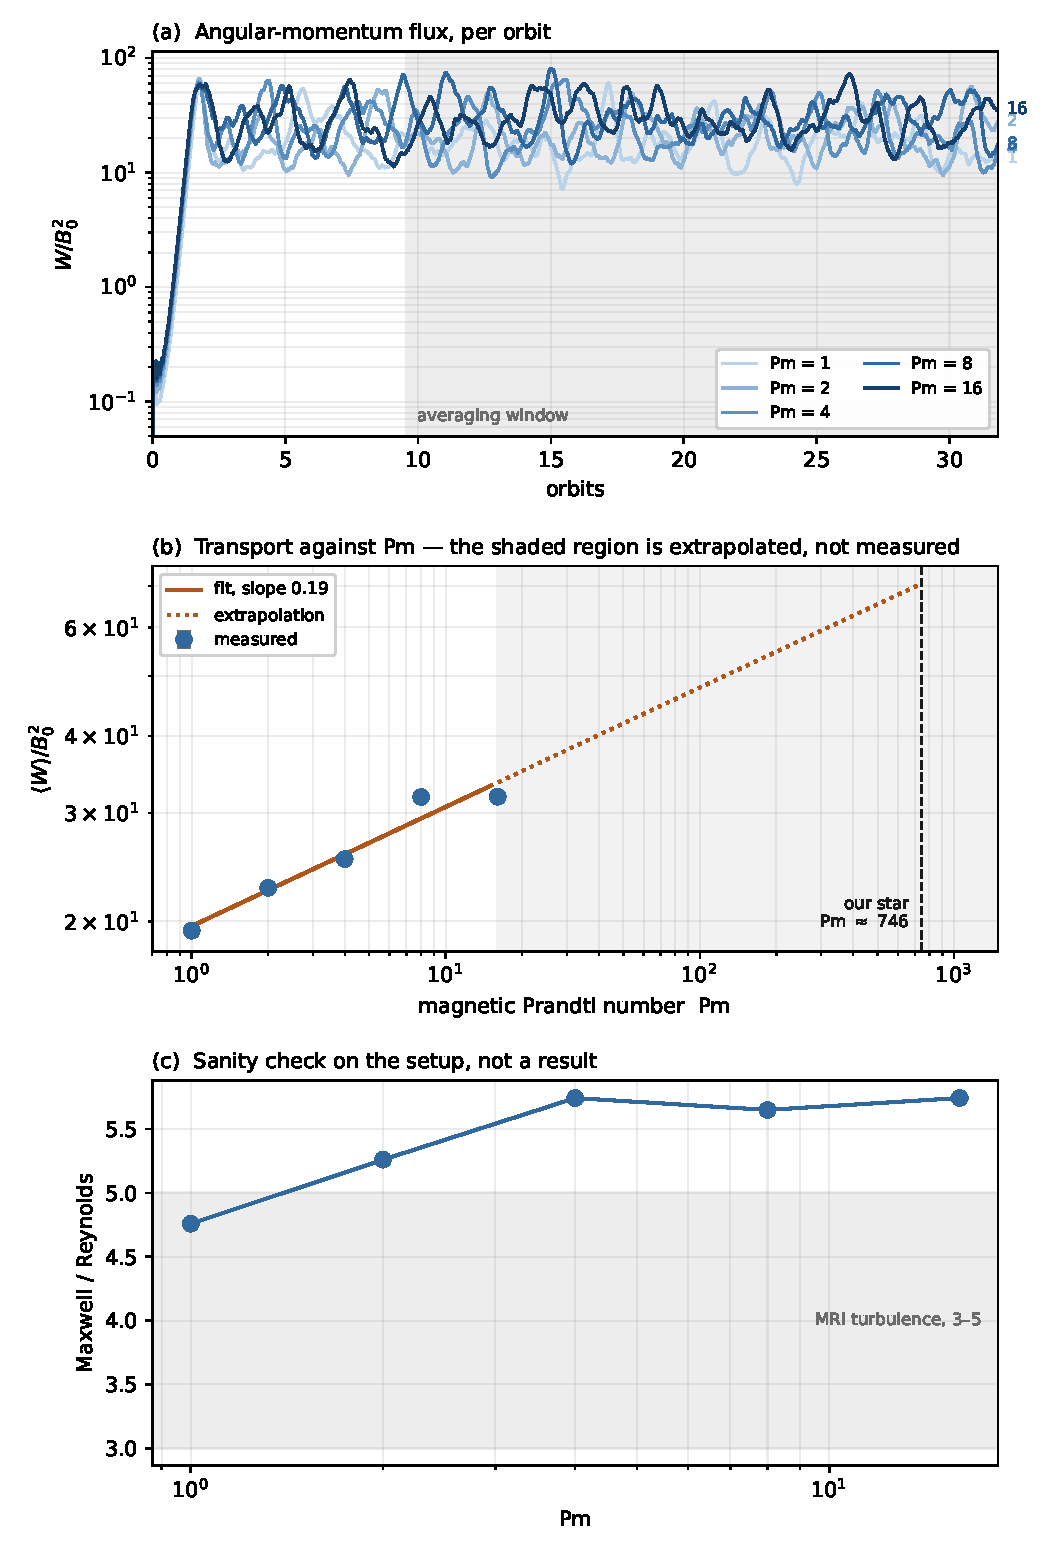
\includegraphics[width=0.70\textwidth]{figures/pm_scan.pdf}
\caption{\textbf{(a)} All five saturate within about two orbits and sustain
turbulence for thirty; the shaded band is the averaging window. \textbf{(b)}
Transport rises as $\Pm^{0.19}$, but the top two points coincide; the shaded
region to the right is \emph{extrapolated, not measured}. \textbf{(c)} The
Maxwell/Reynolds ratio, a check on the setup rather than a result. Data:
\texttt{shearing\_box/analyse\_pm\_scan.py}.}
\label{fig:scan}
\end{figure}

\subsection{The fit, and a correction to our own pre-registered criterion}

The five points fit $W/B_0^2 = 19.7\,\Pm^{0.194}$.

Before the runs started, a sanity criterion was registered: the literature finds
slopes of $0.5$--$1$, so a slope near zero or negative would indicate a setup
error rather than interesting physics. \textbf{That criterion was wrong.}
\citet{lesur2007} give $\delta$ in the range $0.25$--$0.5$ over
$0.12 < \Pm < 8$ and $200 < \Rey < 6400$. The $0.5$--$1$ had been taken from a
search summary and recorded as though verified.

Against the correct band our $0.19$ sits just below --- same sign, same order.
That is acceptable for a single unvalidated resolution, but it is not agreement
and is not reported as such.

\subsection{The flattening, which is the real finding}

$\Pm = 8$ and $\Pm = 16$ agree to $0.039$ against a $2\sigma$ of $0.92$. Two
readings are consistent with the data and it does not separate them:

\begin{enumerate}\itemsep2pt
\item $\alpha(\Pm)$ genuinely saturates above $\Pm \sim 8$. This is plausible
      and untested --- \citet{lesur2007} stopped at exactly $\Pm = 8$.
\item At $64^3$ numerical resistivity already dominates, so the code cannot
      distinguish $\Rm = 8000$ from $\Rm = 16000$. This possibility was recorded
      before any numbers existed, and it fired.
\end{enumerate}

The test that separates them is one run at $128^3$ and $\Pm = 16$: if $W$ rises,
the $64^3$ point was resolution-limited. It costs roughly $16\times$ a $64^3$
run and has not yet been done.

%======================================================================
\section{The implied braking time, and why it is uncomfortable}

Equation~\eqref{eq:alpha} can be evaluated with the star's own numbers, and the
result is the sharpest statement this report contains. Using the measured
late-time volume-typical poloidal field $B_{\mathrm{pol,rms}} = 7\times10^{10}$\,G,
so $B_z \simeq 5\times10^{10}$\,G, and the degenerate pressure at the run's mean
density, $P = 7.8\times10^{24}$\,erg\,cm$^{-3}$:

\begin{table}[h]
\centering\small
\begin{tabular}{lr}
\toprule
plasma $\beta$ on the vertical field & $8\times10^{4}$ \\
$W/B_0^2$ at the top of the scan & $32$ \\
implied $\alpha$ & $8\times10^{-4}$ \\
turbulent viscosity $\nu_t = \alpha c_s H$, $H \sim \Req$ & $7.6\times10^{14}$\,cm$^2$/s \\
\midrule
\textbf{braking time} $\Req^2/\nu_t$ & $\mathbf{\sim 130\ \mathrm{s}}$ \\
\textbf{length of our longest run} & $\mathbf{78\ \mathrm{s}}$ \\
\bottomrule
\end{tabular}
\caption{Order of magnitude only --- see the caveats below. The two rows that
matter are the last two.}
\label{tab:brake}
\end{table}

\subsection{Done properly: an actual torque}

$H \sim \Req$ was the crudest input in that chain and the conclusion is sharp
enough to be worth replacing. The turbulent stress exerts a torque across the
cylinder separating the inner half of the mass from the outer half, so the
inner region redistributes its angular momentum on
\begin{equation}
  \tau = \frac{L_{z,\mathrm{inner}}}{G(r_{1/2})},
  \qquad
  G = 2\pi r_{1/2}^2\, Z(r_{1/2})\, W,
  \qquad
  W = \Big(\tfrac{W}{B_0^2}\Big)_{\!\mathrm{box}} \frac{B_z^2}{4\pi},
\end{equation}
with $L_{z,\mathrm{inner}}$, $r_{1/2}$ and the shell definitions taken from the
diagnostic itself and $Z$ the star's vertical extent there. A second
improvement comes with it: $r_{1/2} = 0.26\,\Req$, where the Komatsu law gives
$q = 0.47$, and the $q$ scan measures $W/B_0^2 = 18.1$ there rather than the
$32$ of Keplerian shear.

This gives $\tau = 557$\,s, or $293$--$428$\,s once the $\Pm$ correction is
folded in --- \textbf{four times longer than the envelope}. So the sharpest
version of the claim, that the rotation should already have been erased inside
our run, does not survive doing the calculation properly.

\subsection{What replaces it, and it is sharper}

The comparison that decides the question is not against the star's total
angular-momentum loss, which is $L_z$ leaving the star altogether and a
different thing from internal redistribution. It is against the observed rate
of change of the \emph{inner} region's angular momentum, since that and the MRI
torque are both the rate at which $L_z$ crosses $r_{1/2}$.

\begin{table}[h]
\centering\small
\begin{tabular}{lrr}
\toprule
over $t = 30$--$78$\,s & & \\
\midrule
observed $\mathrm{d}L_{z,\mathrm{inner}}/\mathrm{d}t$ & $+4.21\times10^{46}$ & erg \\
observed $\mathrm{d}L_{z,\mathrm{outer}}/\mathrm{d}t$ & $-1.35\times10^{47}$ & erg \\
\midrule
predicted MRI torque $G$ & $5.59\times10^{46}$ & erg \\
\bottomrule
\end{tabular}
\caption{The inner region \emph{gains} angular momentum while the outer loses
it: transport is inward, which is the steepening. The MRI would drive it
outward.}
\label{tab:torque}
\end{table}

\textbf{The predicted MRI torque is $1.3$ times the observed inward transport,
and opposite in sign.} That is the result: not that the MRI would have erased
the differential rotation, but that it is a \emph{leading-order competing
effect} of the same size as the transport producing the steepening, pointing
the other way. Switching it on could plausibly cancel the steepening rather
than merely dent it, and the sign of the outcome is not predictable from
anything measured here.

This is consistent with \citet{miravet2025}, who switch on a subgrid MRI
closure in a differentially rotating magnetised neutron star and find the inner
profile flattening where we find it steepening.

\paragraph{Two things the late window adds.} Past $60$\,s the inner region stops
gaining --- $\mathrm{d}L_{z,\mathrm{inner}}/\mathrm{d}t$ falls to
$-1.5\times10^{44}$, essentially zero --- while the outer keeps losing. The
steepening continues at half its earlier rate, $-0.32$ against
$-0.62\%$\,s$^{-1}$, but it is now driven by the outer region shedding angular
momentum rather than the inner gaining it. Those are different mechanisms and
only the first competes directly with the MRI.

\paragraph{What still limits the estimate.} $B_z$ is taken uniform at the
volume-typical value, and $\alpha \propto B_z^2$; if the field is weaker at
$r_{1/2}$ than on average, the torque falls and $\tau$ rises. $r_{1/2}$ is
imported from the $192^3$ diagnostic, which carries it where the $256^3$ CSV
does not. And the field itself is the decayed late-time one, which Report~II
shows is not converged. A factor of a few either way remains.

%======================================================================
\section{What this says about the star, and what it does not}

Relative to $\Pm = 1$, the transport at the stellar $\Pm \approx 750$ is a
factor $3.7$ if the trend continues and $1.6$ if it has already saturated.
\textbf{A factor of a few in either case, not orders of magnitude.} That is
itself useful: what decides the fate of the differential rotation is the value
of $\alpha$, not the Prandtl number, and the high-$\Pm$ correction is a modest
one.

Three limitations bound all of the above.

\begin{enumerate}\itemsep2pt
\item \textbf{The extrapolation is real and is $1.7$ decades wide.} No direct
      numerical simulation reaches $\Pm = 750$, which would need
      $\Rm = 750\,\Rey$ and so $\Rm \sim 10^6$ at any resolvable $\Rey$. The box
      brackets rather than matches. It is a lower bound only if the trend does
      not saturate --- and our own top two points suggest it may.
\item \textbf{The box does not remove extrapolation, it moves it} from $\beta$
      to $(\Rm, \Pm)$. A direct simulation reaches $\Rm \sim 10^3$--$10^4$
      against the star's $10^{20}$. The gain is that this is one extrapolation
      in a named parameter whose direction is known, instead of several that
      were not.
\item \textbf{Nothing here touches the field.} The box has no curvature and so
      no Tayler instability, and the subgrid model these coefficients would feed
      enters the momentum equation only, not the induction equation. The
      destruction of the ordered field reported in Reports~I and II remains
      without a counterpart calculation.
\end{enumerate}

%======================================================================
\section*{Next}

\begin{enumerate}\itemsep2pt
\item $128^3$ at $\Pm = 16$, to decide whether the flattening is physics or
      resolution. It is the one result above that is currently ambiguous.
\item Scan $q$ over $0$--$2$, the range our Komatsu rotation law spans, now that
      the Keplerian check has been made.
\item Scan the net toroidal-to-vertical flux ratio, which in our star runs from
      $2$ to $9.5$ in amplitude. This is the configuration MInIT's
      vertical-field MRI does not obviously describe, and the box can test which
      instability dominates at our ratio.
\item Extract the closure coefficients and compare with the published
      $\alpha^{\mathrm{PI}} = -1.4$, $\beta^{\mathrm{PI}} = -0.8$.
\end{enumerate}

\vspace{0.6em}
\noindent
Code, inputs and analysis are under version control in the \texttt{WD\_MAG}
repository, under \texttt{shearing\_box/}. SNOOPY v6.0 is GPL-3.0 and is not
redistributed there; \texttt{build.sh} reproduces the build, including its FFTW
dependency, without root.

\begin{thebibliography}{9}
\bibitem[Lesur \& Longaretti(2007)]{lesur2007}
Lesur, G., \& Longaretti, P.-Y. 2007,
\textit{Impact of dimensionless numbers on the efficiency of
magnetorotational instability induced turbulent transport},
MNRAS, 378, 1471.
\bibitem[Shternin(2008)]{shternin2008}
Shternin, P.~S. 2008,
\textit{Shear viscosity of degenerate electron matter},
J.\ Phys.\ A: Math.\ Theor., 41, 205501.
\bibitem[Miravet-Ten\'es et al.(2025)]{miravet2025}
Miravet-Ten\'es, M., Obergaulinger, M., Cerd\'a-Dur\'an, P., Font, J.~A., \&
Ruiz, M. 2025, \textit{Subgrid modelling of MRI-driven turbulence in
differentially rotating neutron stars}, MNRAS, 545, 3.
\end{thebibliography}

\end{document}
